\documentclass[]{spie}  %>>> use for US letter paper
%\documentclass[a4paper]{spie}  %>>> use this instead for A4 paper
%\documentclass[nocompress]{spie}  %>>> to avoid compression of citations

\renewcommand{\baselinestretch}{1.0} % Change to 1.65 for double spacing
 
\usepackage{amsmath,amsfonts,amssymb}
%\usepackage[caption = false]{subfig}
\usepackage{rotating,caption,graphicx,subfig}
\usepackage[colorlinks=true, allcolors=blue]{hyperref}

\begin{document}




%{\centering
%\begin{minipage}{0.55\textwidth}
%  \centering
%  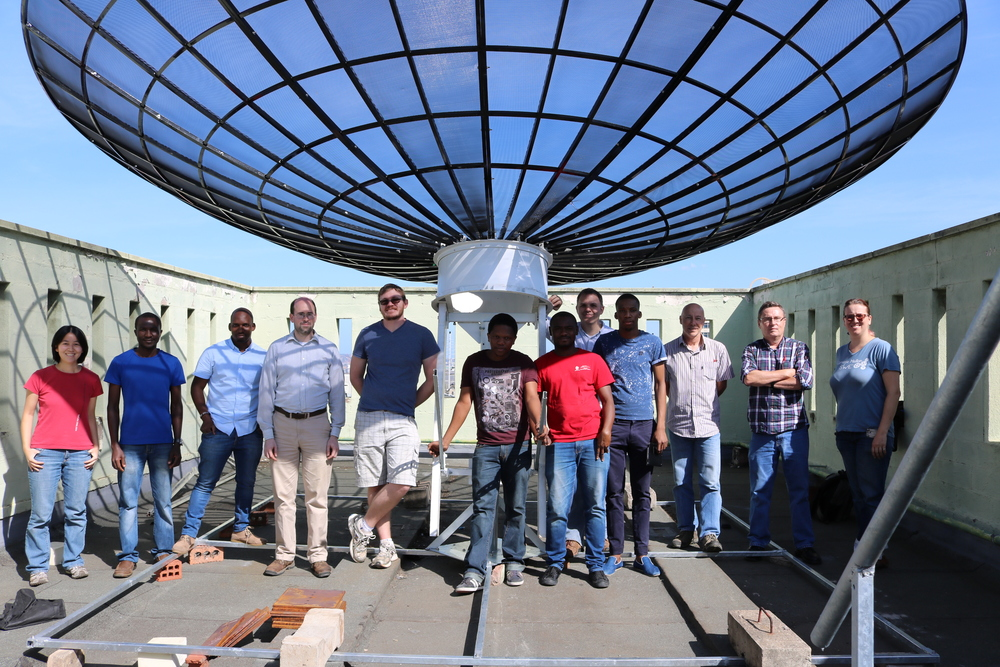
\includegraphics[width=1.0\textwidth]{dish_crew-2.jpg} 
%   \captionof{figure}{The first 6\,m prototype dish for HIRAX was assembled on a rooftop at DUT in Durban, SA.}
%   \captionof{figure}{We are investigating the possibility of amplifying directly on the antenna balun to reduce system noise. This is a prototype with amplifer shown on the stem of the antenna. The amplification circuitry is protected from feed-back and oscillations with a small metal cover.}
%  \label{fig:dishpic}
%\end{minipage}
%\hspace{0.05\textwidth}
%\begin{minipage}{0.35\textwidth}
%  \centering
%   \vspace{0.35in}
%  \rotatebox{-90}{
%   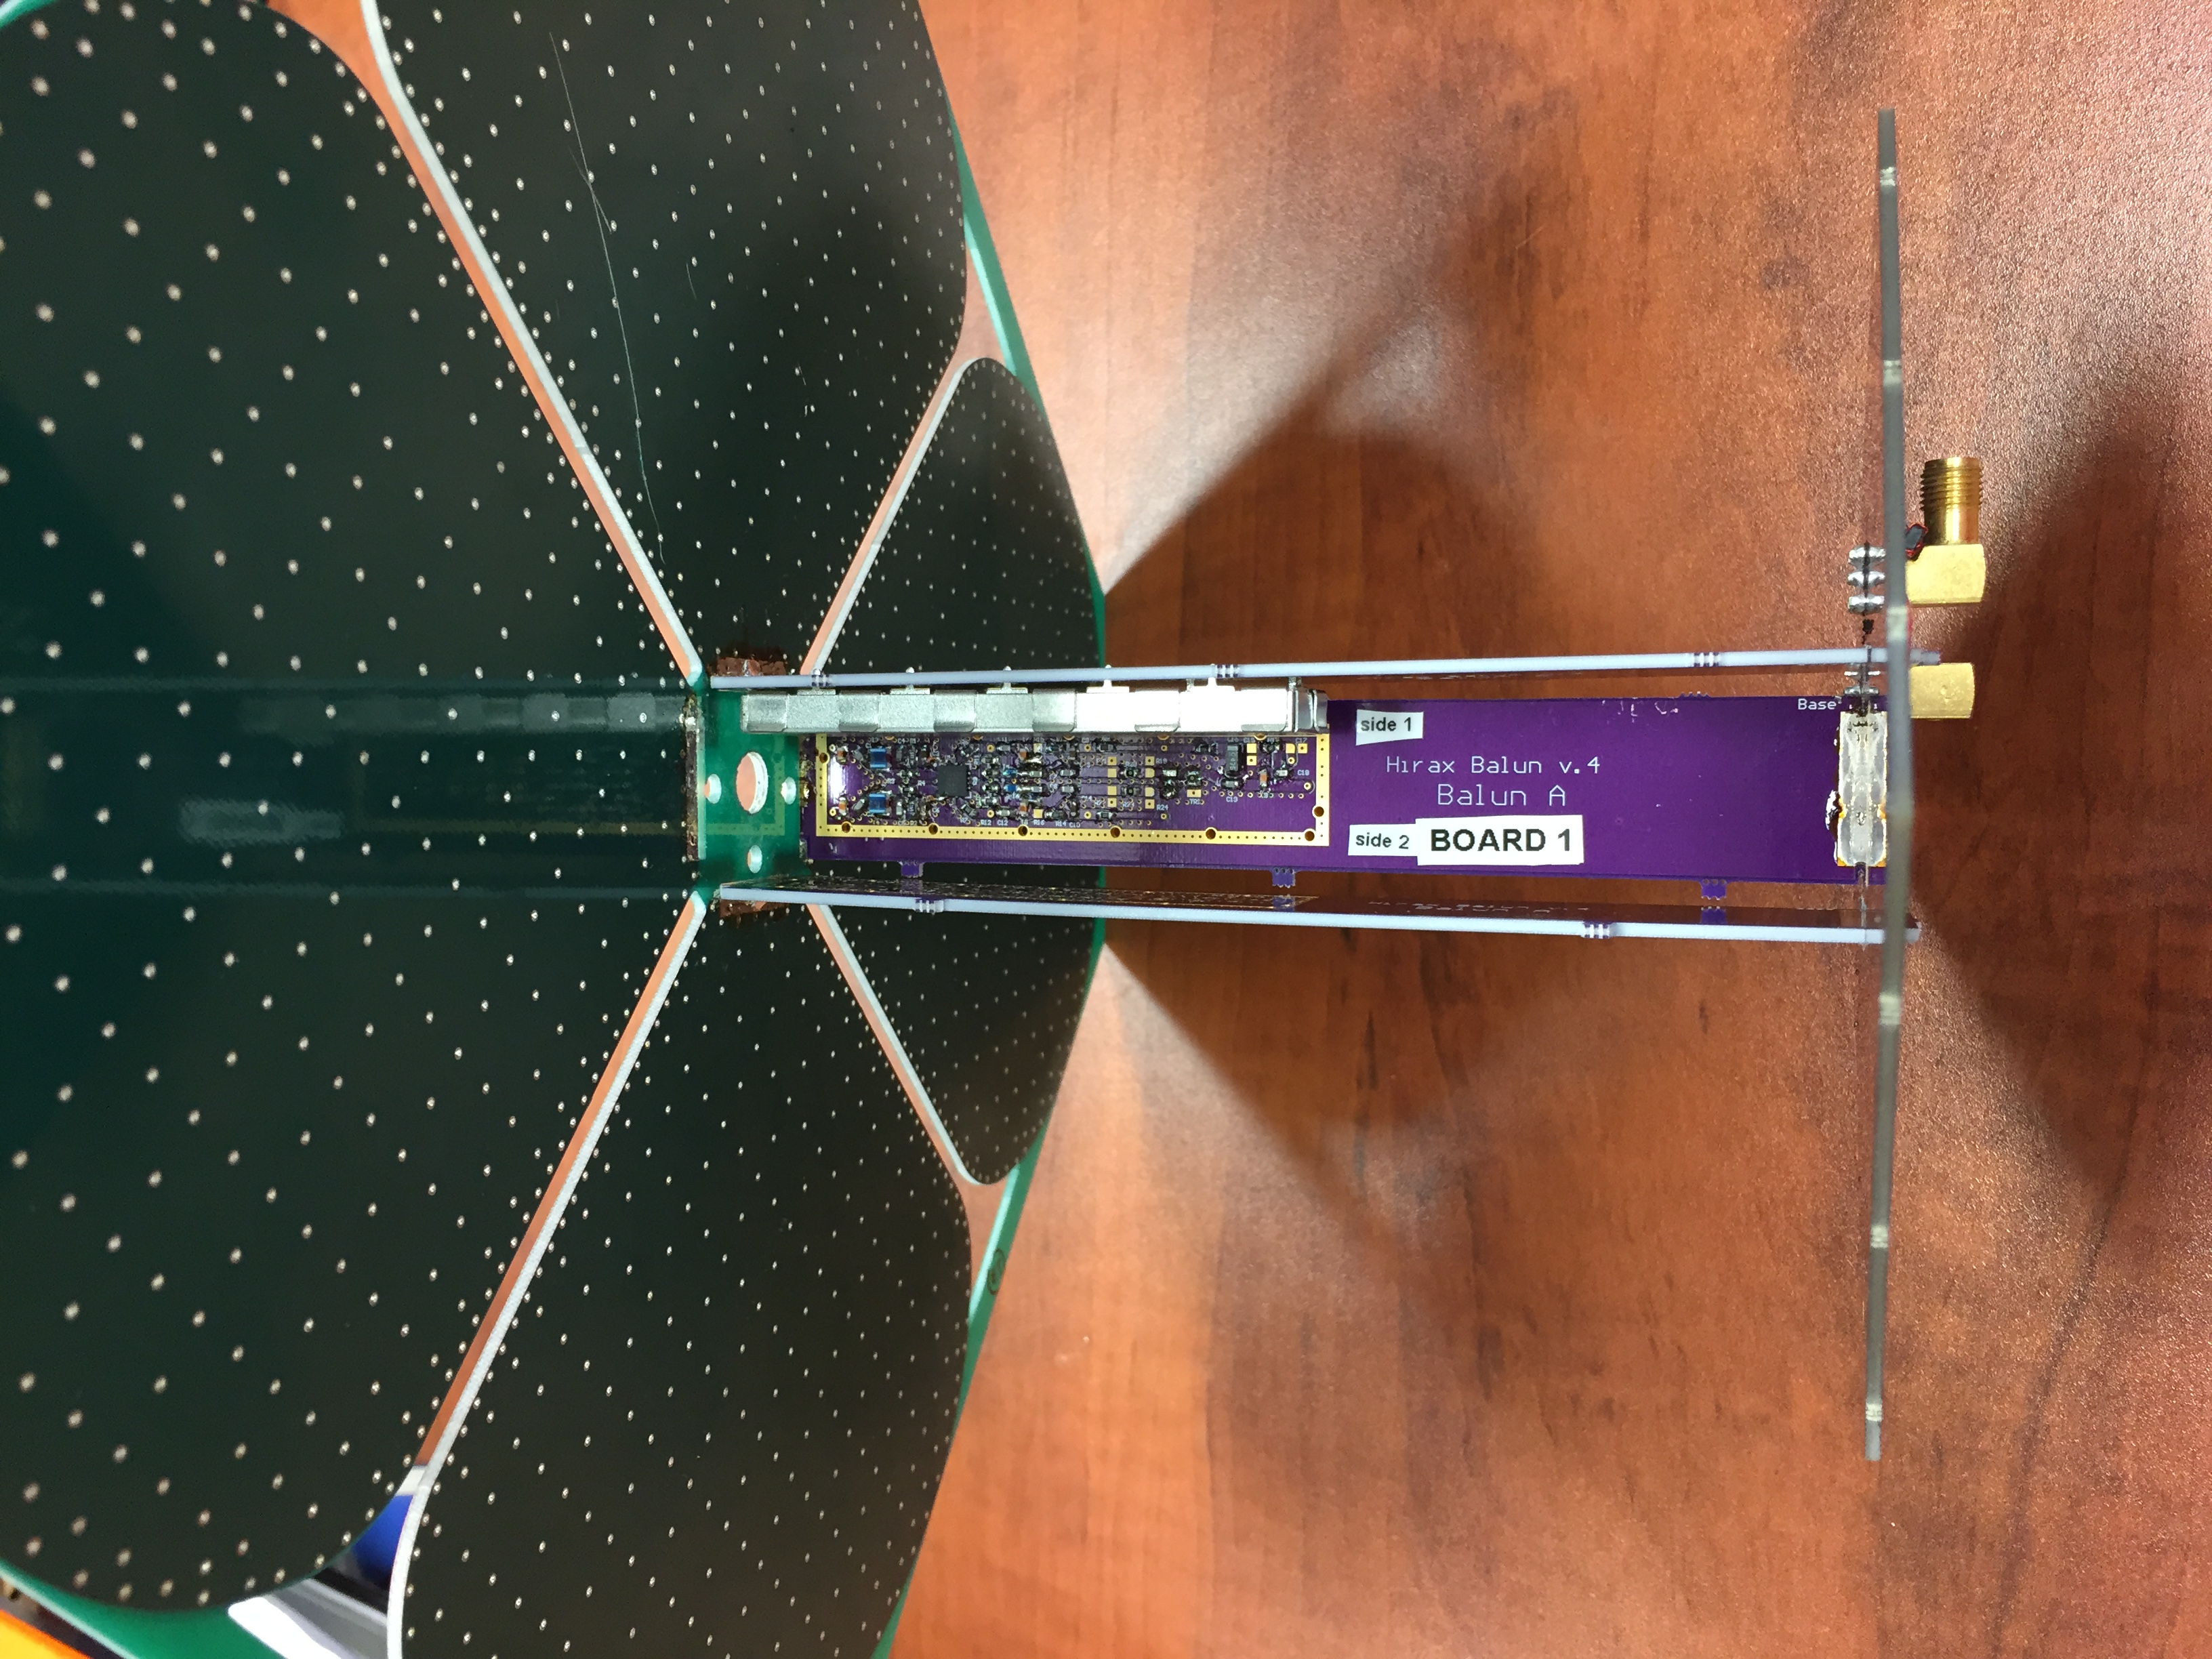
\includegraphics[width=1.0\textwidth]{active_balun.jpg} }
%  \label{fig:activebalun}
%\end{minipage}

\begin{figure}[!tbp]
  \centering
  \begin{tabular}[c]{cc}
    \subfloat[]{\label{fig:dishpic}%
      \begin{tabular}[c]{c}
        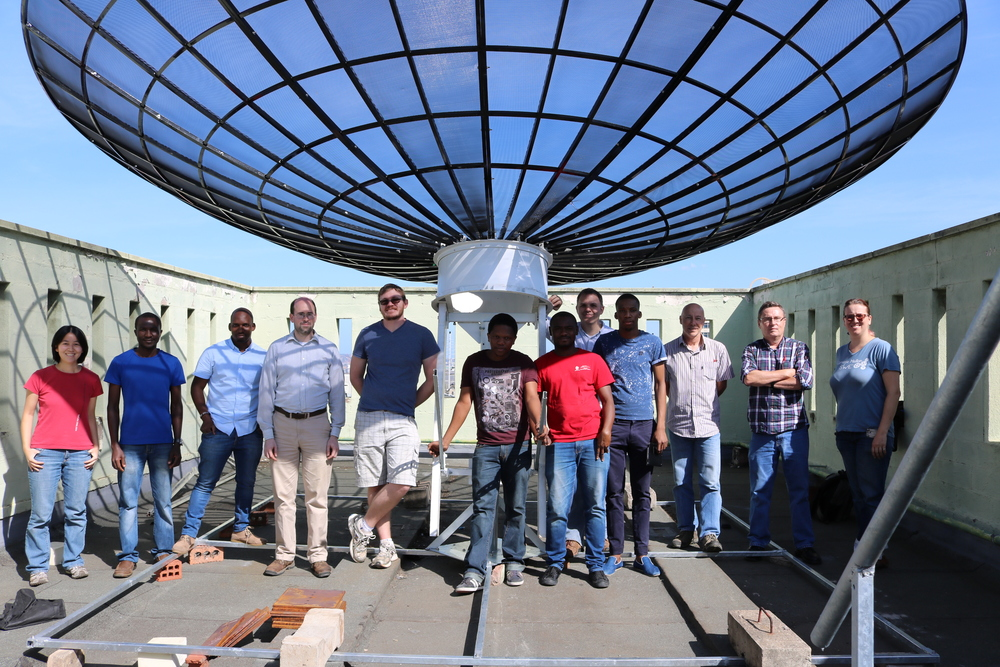
\includegraphics[width=0.6\textwidth]{dish_crew-2.jpg}
      \end{tabular}}
    &
    \begin{tabular}[c]{c}
      \subfloat[]{\label{fig:activebalun}%
         \rotatebox{-90}{
        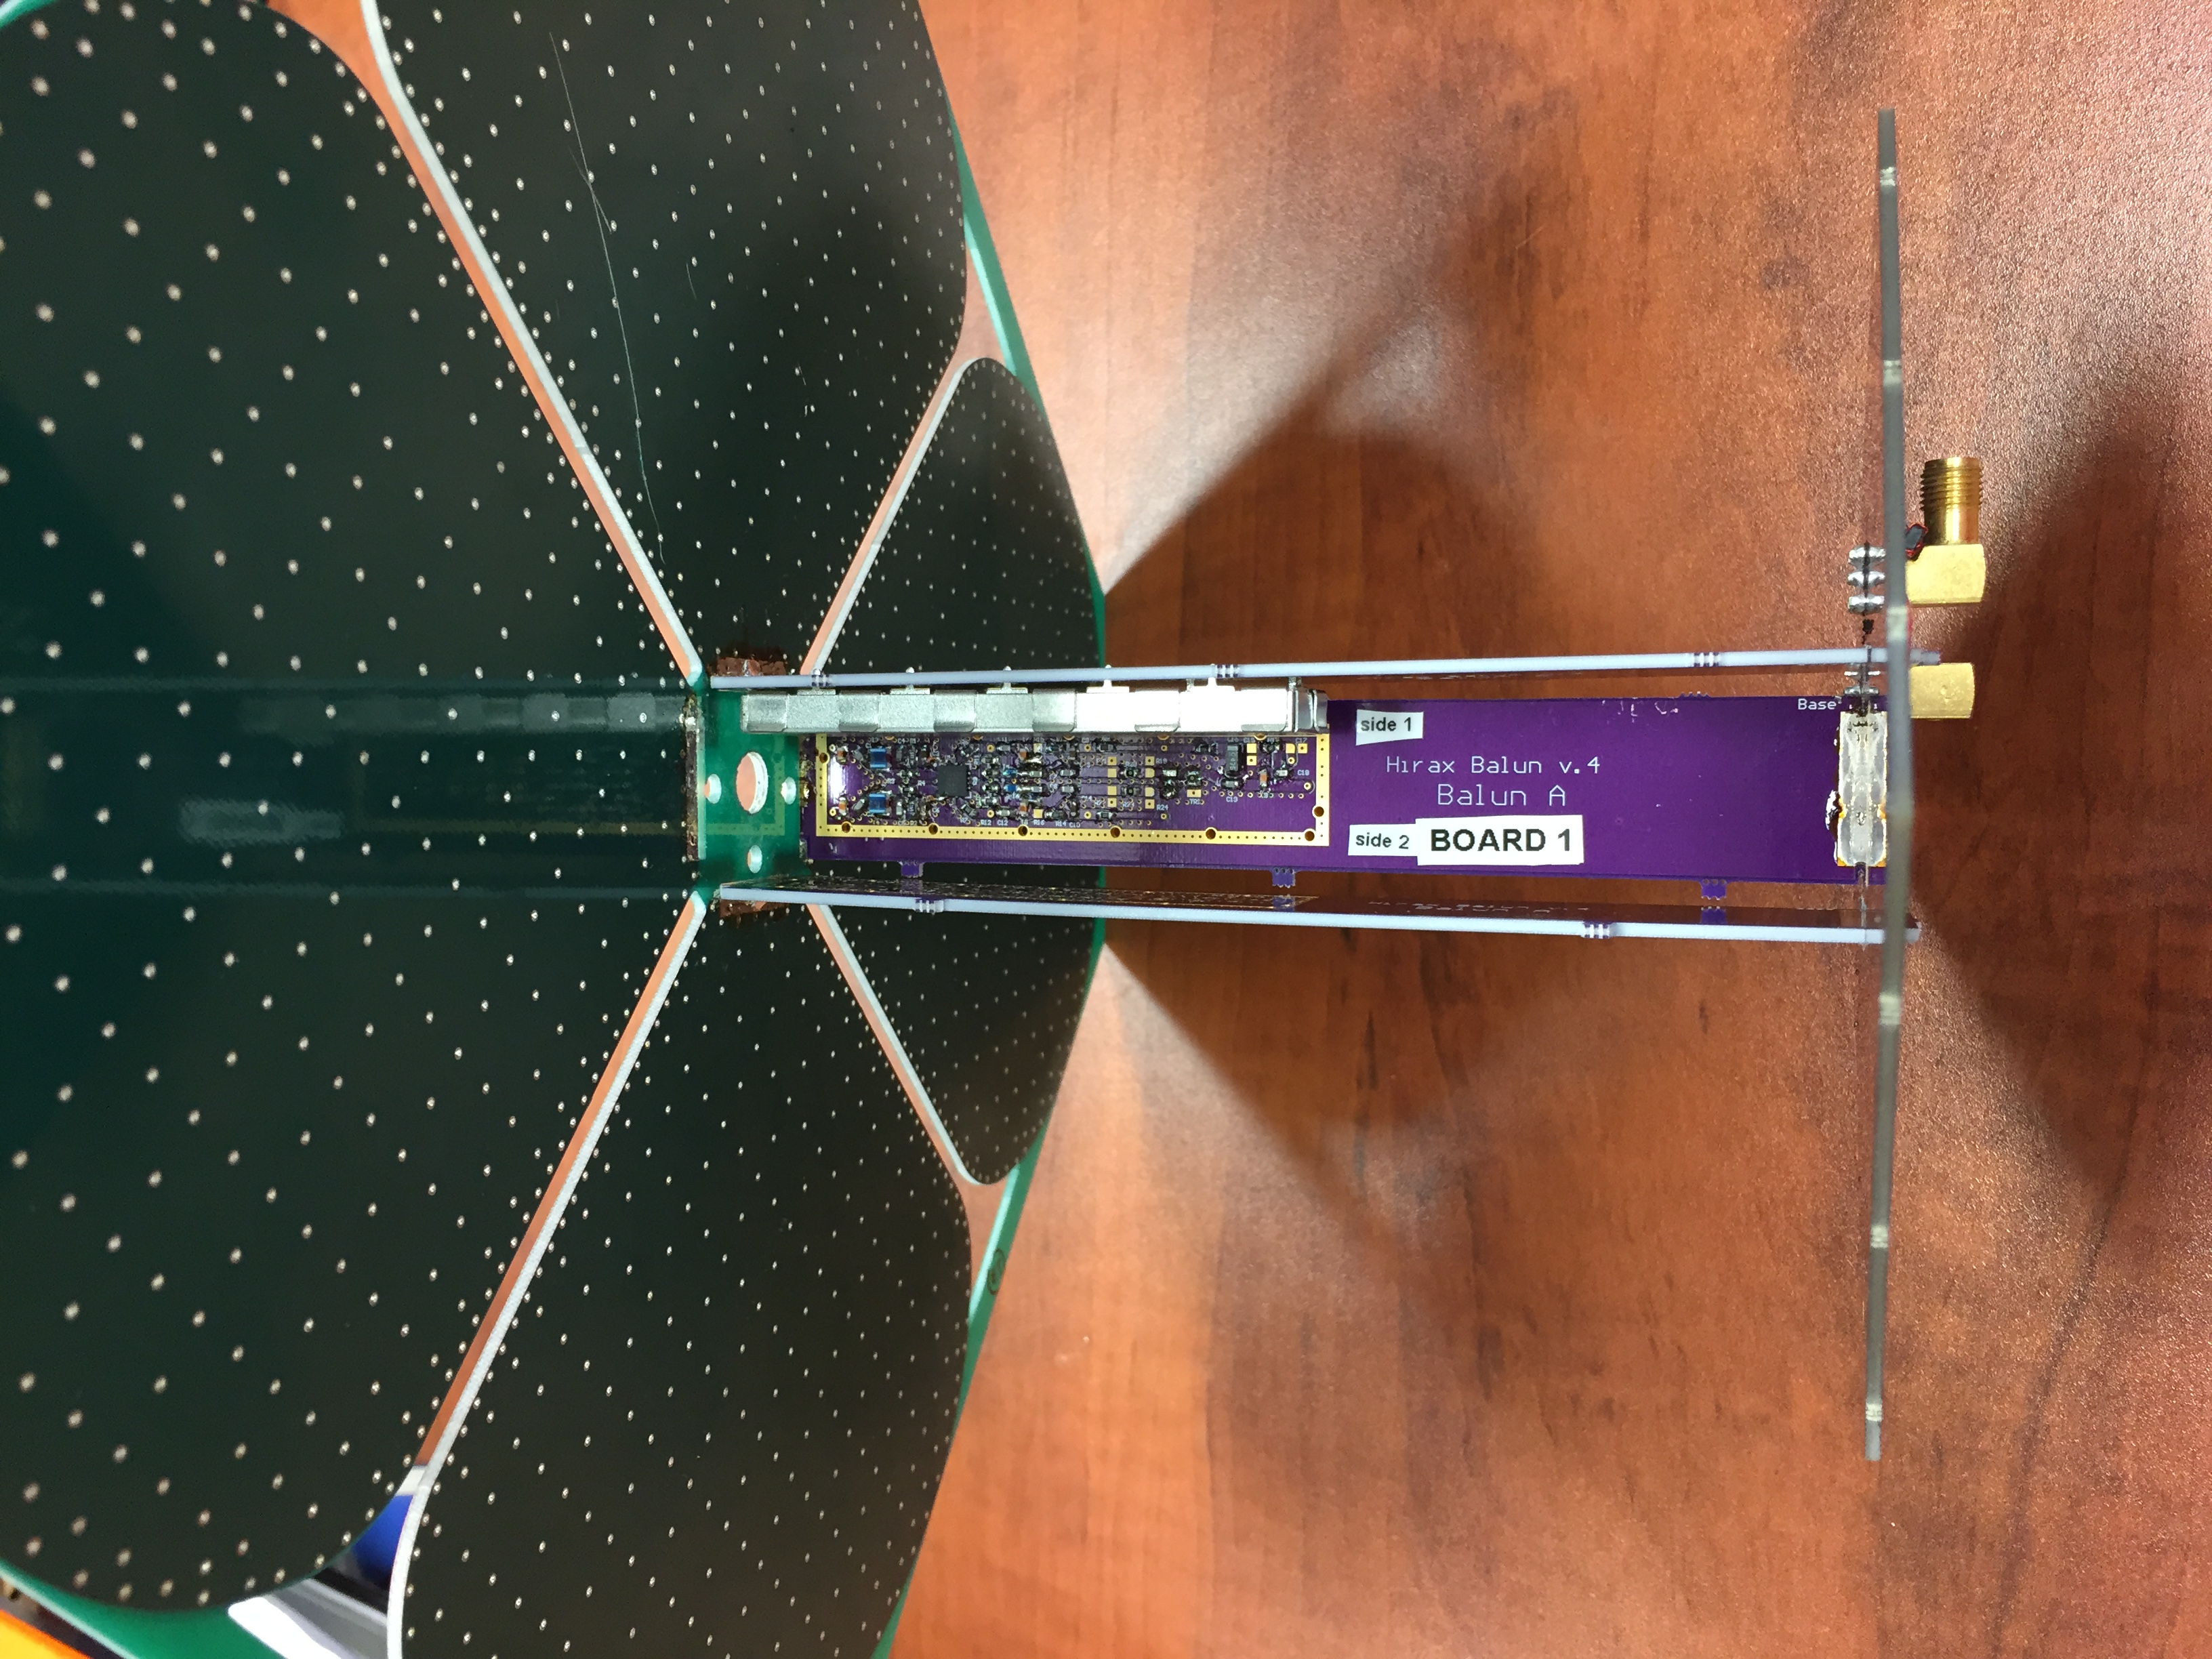
\includegraphics[width=0.35\textwidth]{active_balun.jpg}}}
    \end{tabular}
  \end{tabular}
  \vspace{0.2in}
  \caption{(a) The first 6\,m prototype dish for HIRAX was assembled on a rooftop at DUT in Durban, SA. (b) We are investigating the possibility of amplifying directly on the antenna balun to reduce system noise. This is a prototype with amplifer shown on the stem of the antenna. The amplification circuitry is protected from feed-back and oscillations with a small metal cover.}
  \label{fig:both}
\end{figure}



\end{document} 
